\begin{marginfigure}[2cm] %MARGIN FIGURE
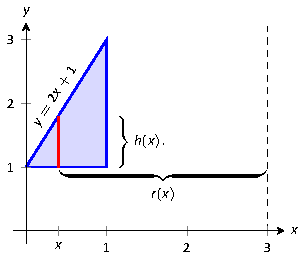
\includegraphics{figures/figshell2a}
\caption{Graphing a region in Example~\ref{eg:6.2.2}.} \label{F:6.2.Ex2a}
\end{marginfigure}

\begin{example} \label{eg:6.2.2} % EXAMPLE
Find the volume of the solid formed by rotating the triangular region determined by the points $(0,1)$, $(1,1)$ and $(1,3)$ about the line $x=3$.

\solution
The region is sketched in Figure \ref{F:6.2.Ex2a} along with the differential element, a line within the region parallel to the axis of rotation. 

The height of the differential element is the distance from $y=1$ to $y=2x+1$, the line that connects the points $(0,1)$ and $(1,3)$. Thus $h(x) = 2x+1-1 = 2x$. The radius of the shell formed by the differential element is the distance from $x$ to $x=3$; that is, it is $r(x)=3-x$. The $x$-bounds of the region are $x=0$ to $x=1$, giving
\begin{align*}
V &=	2\pi\int_0^1 (3-x)(2x)\ dx \\
	&= 2\pi\int_0^1 \big(6x-2x^2)\ dx \\
	&= 2\pi\left(3x^2-\frac23x^3\right)\Big|_0^1\\
	&= \frac{14}{3}\pi\approx 14.66 \ \text{units}^3.
\end{align*}
\end{example}

\begin{marginfigure}[-5cm] %MARGIN FIGURE
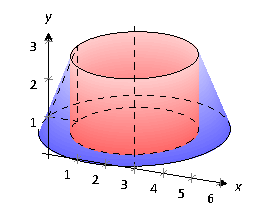
\includegraphics{figures/figshell2b}
\caption{Graphing a region in Example~\ref{eg:6.2.2}.} \label{F:6.2.Ex2b}
\end{marginfigure}